%*******************************************
\section{Target Group}
%*******************************************
\label{s:target_group}

\subsection{Target Group definition}
In this section we want to describe the targeted users for our app.
The main condition that must be met is that they can learn something from our app.
That means they are skilled enough to use the app and not to skilled so that they already know everything that the app tells them.
In detail this is modelized by the following conditions.
\begin{description}[leftmargin=0cm]
\item[Attackabilty] The first precondition is that all our users must meet is that they are possible targets for phishing.
This means they must use the Internet.
They also should use the Internet often enough and have a common trust in the web so that they are in general willing to enter their personal data.
\cite{divsi2012divsi}
\item[Android users] The second precondition is that they should use a android smartphone.
Our evaluation shows that the app is also usable by iOS users but they are not the target group because they can not use the app on a regular basis.
\item[Language] The informative parts of our app are texts and they are written in german.
This means the target user should be able to read german texts.
\item[Motivation] The distribution plan for this app is to put it on the google play store and hope that users download and install it.
Therefore the target user must be willing to learn something about the internet.
\cite{divsi2012divsi} shows that some internet users are so sure about their knowledge that they are not willing to learn something.
We will not be able to reach these users.
\end{description}

\subsection{Projection to Population}
After we have roughly decided what our target group is we wanted to be sure that we don't rule out to much of the population with these preconditions.
This means it is of no use to produce a app that is, after all, only of use for 1 \% of the population.
To proof this we looked at a big survey done by SINUS-Instituts Heidelberg in behalf of Deutschen Instituts f\"{u}r Vertrauen und Sicherheit im Internet (DIVSI).
This survey first looked at 60 persons in detail and found seven types of internet users.
Thereafter they tried to apply the findings to the whole german population by interviewing 2,000 representative persons.
We tried to match our preconditions to these groups. Following is our evaluation for each group\cite{divsi2012divsi}.

\begin{figure}[hHtbp]
\centering
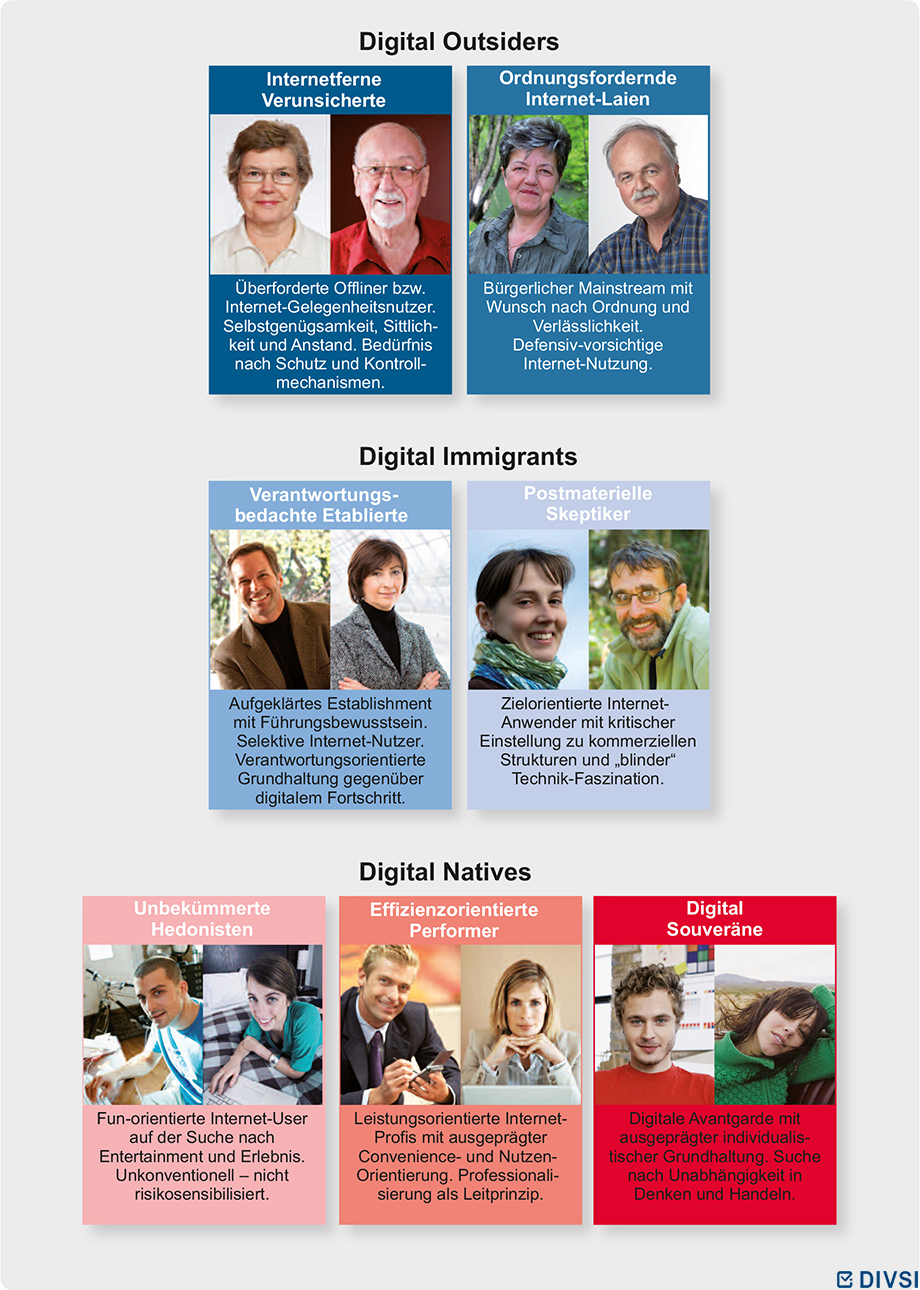
\includegraphics[width=0.56\textwidth]{graphix/DIVSI-Milieus.jpg}
\caption{Internet Milleus as defined by DIVSI}
\label{fig:divsi_milieus}
\end{figure}

\begin{description}[leftmargin=0cm]
\item[Digital Souver\"{a}ne] This group moves naturally in the internet and is therefore exposed to phishing. They also often use smartphones. We rule them out because because they think that they already know the problems of the internet so they need to be trained. Therefore they will probably never download the app.
\item[Effizienzorientierte Performer] This group matches our preconditions because they are using the internet naturally as well as smartphones. In contrast to the previous group the are interested in learning something new and see their own learning in an investment into the future. To target this group we should show that you can learn something from this app.
\item[Unbek\"{u}mmerte Hedonisten] This group is also native in the digital worlds but in contrast to the before mentioned groups are not aware of the problems and frauds therein. When they are aware of the problems they seek to secure themselves with automated software and are not interested in investing time therein. Therefore they are not motivated to use our app.
\item[Postmaterielle Skeptiker] This group is interested in the internet and uses it frequently. On the other hand they are aware that there are problems and frauds. As they are interested in information in the internet especially from official sources they might download our app. To target this group we should clearly state that this app is from an university.
\item[Verantwortungsbedachte Etablierte] This group uses the internet regulary and also use smartphones. They are exspecially interested in using protection software and actively search information in the internet. The users of this group don't think that they could protect themselves from the dangers of the internet and actively seek to change this. Therefore they mostlikely will find the app. To target this group we should clearly state that this app protects the user.
\item[Ordnungsfordernde Internet-Laien] These users are using the internet very infrequently. Because of this they are very careful when using the internet and normally don't enter personal data. Therefore it is not likely that they will use the app. Also they mostly don't have smartphones.
\item[Internetferne Verunsicherte] These users don't use the internet. Therefore they are not exposed to phishing threads.
\end{description}

\begin{figure}[hHtbp]
\centering
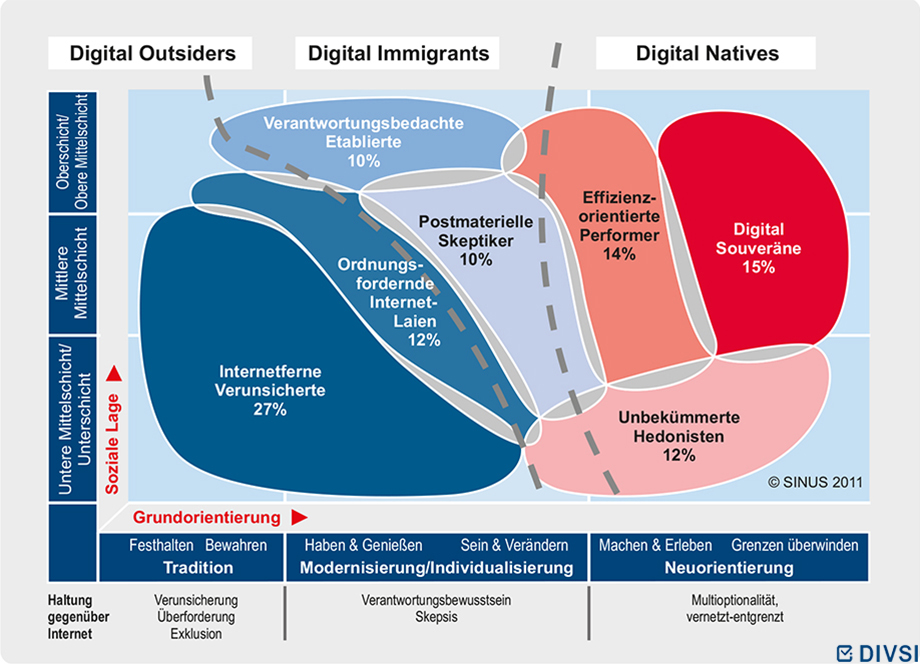
\includegraphics[width=0.56\textwidth]{graphix/DIVSI-Kartoffeln.jpg}
\caption{Internet Milleus as defined by DIVSI}
\label{fig:divsi_kartoffeln}
\end{figure}

In Conclusion we consider \textit{Verantwortungsbedachte Etablierte} (10\%),  \textit{Postmaterielle Skeptiker} (10\%),  \textit{Effizienzorientierte Performer} (14\%). In total these are 34\% of the german population.